\section{Aufbau und Durchführung}
\label{sec:Durchführung}

\subsection{Aufbau}

\noindent Der Aufbau des Sagnac-Interferometers ist schematisch in der \autoref{fig:Interferoa} dargestellt. Der benutzte HeNe - Laser emittiert Licht der 
Wellenlänge $\SI{632.99}{\nano\metre}$ \cite{anleitung}, dieses Licht wird über die Spiegel $M_1$ und $M_2$ auf einen Polarizing Beam Splitter Cube (PBSC) reflektiert. 
Dort wird ein Teil des Lichtstrahls reflektiert und läuft im Uhrzeigersinn durch das Interferometer und ein anderer Teil des Lichtstrahls wird 
transmittiert und läuft entgegen des Uhrzeigersinnes durch das Interferometer. Nach einem Umlauf werden die Lichtstrahl durch den PBSC wieder zusammengeführt. In der 
\autoref{fig:Interferob} ist vor dem PBSC ein Polarisationsfilter zu sehen, welcher mit dem Winkel $\phi$ ausgelenkt ist und in der Kontrastmessung gebraucht wird. 
Außerdem soll dieser feststellen, dass hinter dem PBSC der vertikalpolarisierte und horizontalpolarisierte Anteil des Lichtstrahls gleichermaßen vertreten ist, sodass ein Winkel von $\phi = \SI{45}{\degree}$
zur Justage eingestellt wird.  

\begin{figure}[H]
    \centering
    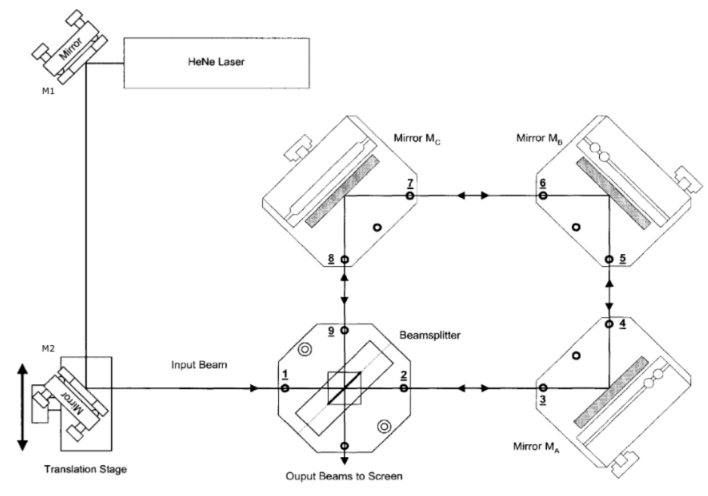
\includegraphics[width=\textwidth]{bilder/Interferometer.png}
    \caption{Der schematische Aufbau des Sagnac-Interferometers. \cite{anleitung}}
    \label{fig:Interferoa}
\end{figure}

% \begin{figure}[h]
    % \begin{subfigure}{0.68\textwidth}
        % \centering
        % 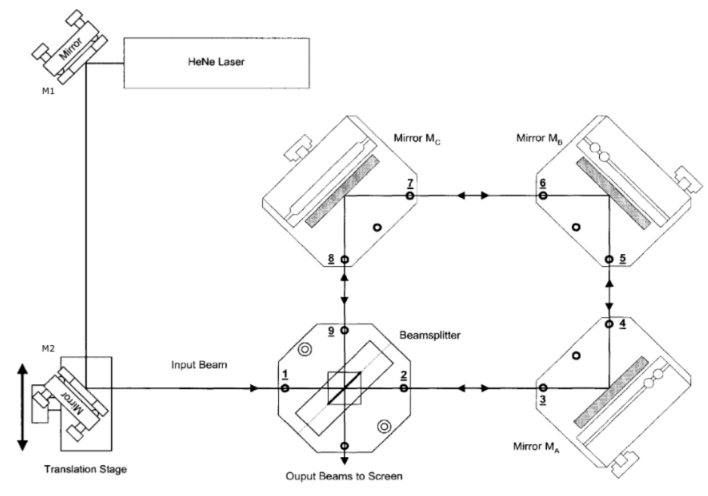
\includegraphics[height=6cm]{bilder/Interferometer.png}
        % \caption{Der schematische Aufbau des Sagnac-Interferometers. \cite{anleitung}}
        % \label{fig:Interferoa}
    % \end{subfigure}
    % \hfill
    % \begin{subfigure}{0.28\textwidth}
        % \centering
        % 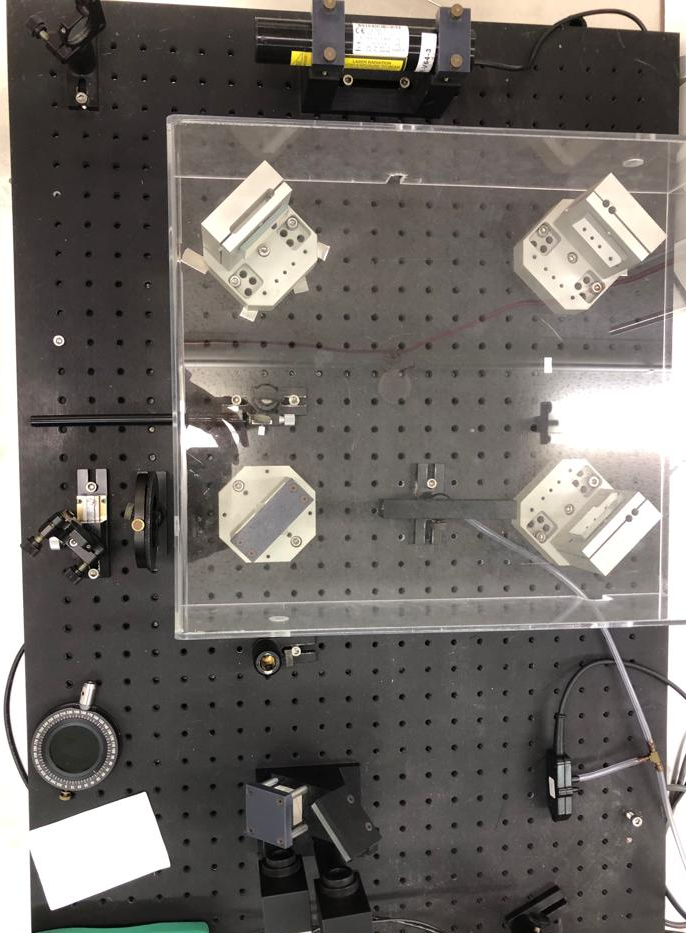
\includegraphics[height=6cm]{bilder/interfer_foto.png}
        % \caption{Der Aufbau des Interferometers im Versuch.}
        % \label{fig:Interferob}   
    % \end{subfigure}
    % \caption{Der Aufbau des Sagnac-Interferometers.}
% \end{figure}

\noindent Eine Eigenschaft des Sagnac-Interferometers ist es, dass die beiden zu interferierenden Strahlen den gleichen Weg durchlaufen. Somit ist das Interferenzbild weniger 
anfällig auf äußere Einflüsse wie Luftdruckschwankungen. Damit eine Messung durchgeführt werden kann, müssen die beiden Lichtstrahlen getrennt werden. Dies passiert durch Bewegen 
des Spiegels $M_2$ parallel zur ersten Oberfläche des PBSC. Die Lichtstrahlen treffen nun an verschiedenen Punkten an den Spiegeln auf, treffen jedoch im PBSC wieder zusammen. 

\begin{figure}[H]
    \centering
    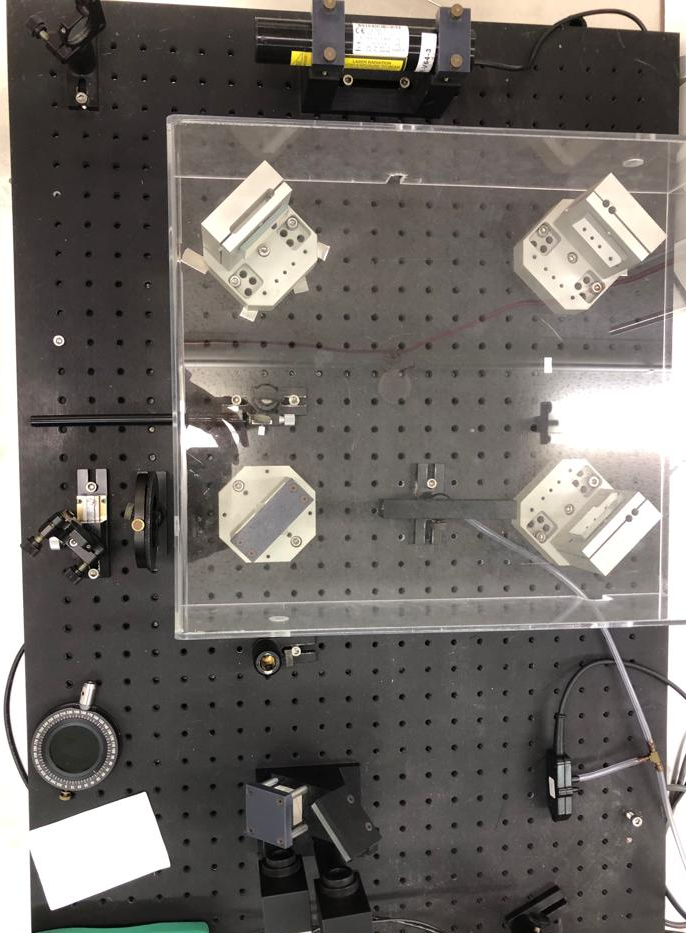
\includegraphics[width=0.5\textwidth]{bilder/interfer_foto.png}
    \caption{Der Aufbau des Interferometers im Versuch. Es ist die Gaskammer im Strahlengang des zuerst vom PBSC transmittierten Strahl zu sehen und der Doppelglashalter im Strahlengang 
    des zuerst reflektieren Strahls. Unten im Bild stehen beide Dioden nebeneinander und der im $\SI{45}{\degree}$ gekippte zweite PBSC ist vor diesen zu erkennen. Der zur Justage benutzte 
    Polarisationsfilter und Schirm liegen vorne links im Bild.}
    \label{fig:Interferob}   
\end{figure}


\noindent Der Output aus dem PBSC zeigt so keine Interferenz auf, da die beiden Strahlen senkrecht zueinander polarisiert sind. Daher wird für die Justage ein Polarisationsfilter mit 
Winkel $\SI{45}{\degree}$ vor einen Schirm gestellt. Die Messung wird mit ein bis zwei Photodioden durchgeführt. Um diese zu nutzen, wird statt des Polarisationsfilter ein um 
$\SI{45}{\degree}$ gekippter PBSC benutzt, wobei der im PBSC reflektierte Strahl nochmal durch einen Spiegel in die Photodiode reflektiert wird. Zur Bestimmung der Anzahl der Maxima 
und Minima wird mit der Differenzmethode gearbeitet, also die Signal der beiden Dioden werden auf ihre Differenz untersucht. Damit werden konstante Störungen wie anderes einfallendes 
Licht aus dem Signal genommen. In der \autoref{fig:Messgeraete} sind die Messgeräte zu sehen, mit denen gearbeitet wurde.

\begin{figure}[H]
    \centering
    \includegraphics[width=\textwidth]{bilder/Messgeräte.png}
    \caption{Die im Versuch benutzten Messgeräte. Im Vordergrund ist links in 
    in einem blau-grün das Multimeter zu sehen, mit welchem die Intensitäten der Minima und Maxima für die Berechnung des Kontrastes gemessen werden.
    Das schwarze stehende Gerät mit gelben Streifen ist das Anzeigegerät des Manometers.Im Hintergrund steht ein Oszilloskop auf einem 
    Modern Interferometry Controller.}
    \label{fig:Messgeraete}
\end{figure}


\subsection{Justage}

\noindent Zu Beginn muss das Sagnac-Interferometer justiert werden. Dies wird mit zwei Justageplatten gemacht, die jeweils 3 Löcher auf der Höhe des Laserstrahls hat. 
Zuerst werden die Spiegel M1 und M2 (siehe \autoref{fig:Interferoa}) so verstellt, dass der durch den PBSC transmittierte Strahl durch das mittige Loch der Justageplatten geht, welche 
auf den Positionen 2 und 3 stehen. Hierbei wird der im PBSC reflektierte Strahl durch einen Schirm blockiert. 
Anschließend werden die Justageplatten an verschiedene Positionen vor den Spiegeln des Interferometers gebracht. Durch Bewegen der Bodenplatte, Erhöhen dieser durch Metallplättchen, 
und Feinjustierschrauben werden beide Strahlen durch das mittlere Loch der Justageplatten geführt. \\
Nachdem ein Polarisationsfilter mit einem Winkel von $\SI{45}{\degree}$ nach dem PBSC eingebaut wird, erscheint auf dem Schirm ein Interferenzmuster. Dieses kann sich noch nicht verändern, 
da keiner der Strahlen einen Phasenverschub erfährt. Die Lichtstrahlen werden nun getrennt durch das Veschieben des Spiegels $M_2$ parallel zur ersten Oberfläche des PBSC. 
Durch Bewegung der Glasplatten, welche im Strahlengang zwischen dem PBSC und dem Spiegel $M_{\text{C}}$ eingebaut werden, werden Interferenzmaxima und -minima durchlaufen.
Im Interferenzmuster sind Streifen zu sehen, welche auftreten, da die Lichtstrahlen nicht perfekt parallel ausgerichtet sind. Durch die Feinjustierschrauben werden diese Streifen 
so gut wie möglich entfernt. 


\subsection{Kontrastbestimmung}
\label{subsec:Kontrastbestimmmung}

\noindent Der Polarisationsfilter und der Schirm werden hinter dem PBSC entfernt, der Outputbeam wird auf einen um $\SI{45}{\degree}$ gekippten weiteren PBSC geleitet, welcher seine beiden
Outputbeam auf zwei Photodioden reflektiert und transmittiert. Eine der Dioden wird an ein Multimeter angeschlossen. Nun wird für verschiedene Werte des Polarisationswinkel $\phi$ des 
Polarisationsfilters vor dem PBSC die Diodenspannung der Interferenzmaxima und -minima gemessen. Die Maxima und Minima werden durch Bewegen des Doppelglashalters eingestellt. Es werden 
in einem Bereich von $\phi \in \left[ \SI{0}{\degree}, \SI{180}{\degree}\right]$ in Schritten von $\increment \phi = \SI{15}{\degree}$ Werte genommen und der Kontrast berechnet. In der Nähe von Winkeln 
mit hohem Kontrast werden Daten im Abstand von $\increment\phi = \SI{5}{\degree}$ genommen.\\
Es wird der Winkel $\phi$ eingestellt, bei dem der größte Kontrast gemessen wurde. Alle weiteren Messungen werden mit dieser Einstellung durchgeführt.


\subsection{Bestimmung des Brechungsindex von Glas}
\label{subsec:n_glas_Durchführung}

\noindent Beide Photodioden werden an den Modern Interferometry Controller angeschlossen, dessen Output wird auf einem Oszilloskop angezeigt. Der Doppelglashalter wird im Bereich von 
$\Theta \in \left[ \SI{0}{\degree}, \SI{10}{\degree}\right]$ bewegt. Der Modern  Interferometry Controller zählt die Nulldurchgänge der Differenz der Diodenspannungen, also die Anzahl 
der Interferenzminima. Diese Anzahl wird für eine ganze Drehung von $\Theta$ um $\SI{10}{\degree}$ gemessen. Die Messung wird $\num{10}$ mal wiederholt.


\subsection{Bestimmung des Brechungsindex von Gas}
\label{subsec:Durchführung_n_Luft}

\noindent Der Doppelglashalter wird aus dem Strahlengang gebaut und eine Gaszelle wird eingebaut. Diese wird mithilfe einer Pumpe leergepumpt. Dann wird kontrolliert Luft in die Gaszelle 
gefüllt und in Schritten von $\SI{50}{\milli\bar}$ die Anzahl der durchlaufenden Interferenzminima notiert. Die Messung wird $\num{4}$ mal wiederholt. Um äußere Einflüsse wie 
Luftdruckschwankungen zu minimieren, wird eine Haube auf das Interferometer gesetzt. 